\documentclass[a4paper, 12pt]{article}

\usepackage{hyperref}
\usepackage[warn]{mathtext}
\usepackage[utf8]{inputenc}
\usepackage[T2A]{fontenc}
\usepackage[english,russian]{babel}
\usepackage{multirow}
\usepackage{amsmath,amsfonts,amssymb,amsthm,mathtools}
\usepackage{indentfirst}
\DeclareSymbolFont{T2Aletters}{T2A}{cmr}{m}{it}
\usepackage{ gensymb }
\mathtoolsset{showonlyrefs=true}
\usepackage{euscript}
\usepackage{mathrsfs}
\usepackage[left=2cm,right=2cm,top=2cm,bottom=2cm]{geometry}
\usepackage{graphicx}
\usepackage{wrapfig}
\usepackage[rgb]{xcolor}
\hypersetup{
colorlinks=true,
urlcolor=blue
}


\title{Лабораторная работа}
\author{Гисич Арсений Б03-102}
\date{2022}

\begin{document}

	\begin{center}
		{\large МОСКОВСКИЙ ФИЗИКО-ТЕХНИЧЕСКИЙ ИНСТИТУТ (НАЦИОНАЛЬНЫЙ ИССЛЕДОВАТЕЛЬСКИЙ УНИВЕРСИТЕТ)}
	\end{center}
	\vspace{5 cm}
	{\Large
		\begin{center}
			{\bf Лабораторная работа 3.1.1}\\[0.2 cm]
			Магнитометр
		\end{center}
	}
	\vspace{4 cm}
	\begin{flushright}
		{\Large Выполнил: \\
			\vspace{0.2 cm}
			Гисич Арсений \\
			\vspace{0.2 cm}
			Б03-102 \\}
	\end{flushright}
	\vspace{9 cm}
	\begin{center}
		Долгопрудный\\[0.1 cm]
		2022
	\end{center}
\thispagestyle{empty}

\section{Аннотация}

В данной работе определялась горизонтальная составляющая магнитного поля Земли и установлено количественное соотношение между единицами электрического тока в системах СИ и СГС.

\section{Теоретические сведения}

Магнитометром называют прибор для магнитных измерений, например: компас, теодолит, веберметр и пр. С помощью магнитометров измеряют намагниченность ферромагнетиков, напряжённость магнитных полей, исследуют магнитные аномалии. Разработаны магнитометры различных конструкций: магнитостатические, электромагнитные, магнитодинамические, индукционные, резонансные. Эталонные магнитометры позволяют измерять горизонтальную и вертикальную составляющие напряжённости магнитного поля Земли с точностью $10^{-6}$ Э.

В нашей установке с помощью электромагнитного магнитометра измеряется горизонтальная составляющая земного магнитного поля и абсолютным образом определяется сила тока по его магнитному действию.

\section{Методика измерений}

Магнитометр (рис.~\ref{ris1}) состоит из нескольких последовательно соединённых круговых витков К, расположенных вертикально. В центре кольца К радиусом $R$ на тонкой неупругой вертикальной нити подвешена короткая магнитная стрелка С. Жёстко связанная со стрелкой крыльчатка погружена в масло и служит для демпфирования колебаний.

\begin{figure}[h!]
\begin{center}
    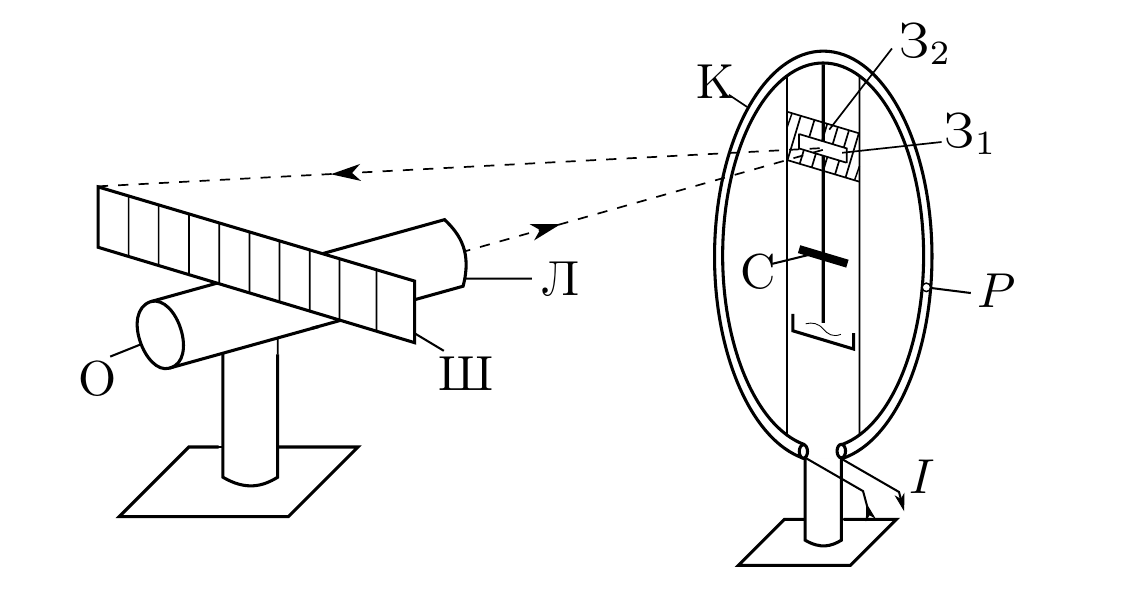
\includegraphics[scale=2.4]{1.png}
\end{center}
\caption{Схема магнитометра}
\label{ris1}
\end{figure}

\begin{figure}[h!]
\begin{center}
    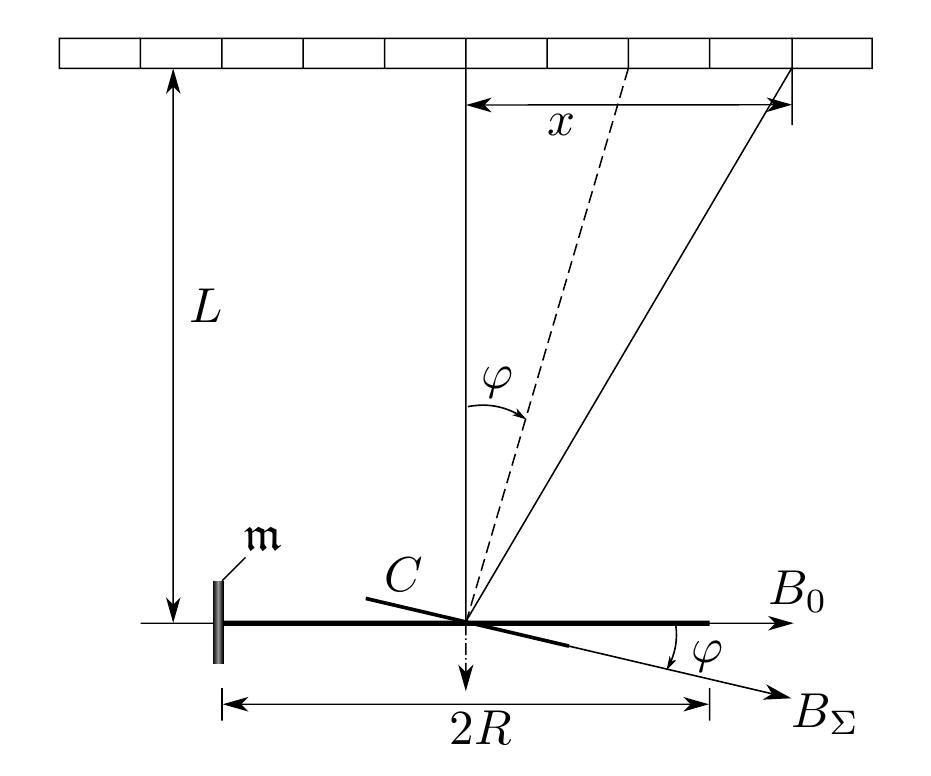
\includegraphics[scale=2.4]{2.png}
\end{center}
\caption{Схема измерения угла отклонения магнитной стрелки}
\label{ris2}
\end{figure}

В отсутствие других магнитных полей стрелка располагается по направлению горизонтальной составляющей земного магнитного поля $B_0$, т. е. лежит в плоскости магнитного меридиана.

Прибор настраивают с помощью световых зайчиков, отражённых от двух зеркал: З1, прикреплённого к стрелке (подвижный зайчик), и З2, расположенного в плоскости кольца К и жёстко связанного с ним (неподвижный зайчик). Оба зеркала освещаются одним и тем же осветителем О. Вращением кольца вокруг вертикальной оси можно совместить оба зайчика. При этом плоскость витков совпадает с плоскостью магнитного меридиана.

При появлении дополнительного горизонтального магнитного поля $B_\perp$ стрелка C установится по равнодействующей обоих полей $B_\Sigma$ (рис.~\ref{ris2}). В нашей установке дополнительное поле может быть создано либо малым ферромагнитным стержнем, расположенным на кольце на его горизонтальном диаметре ($B_1$), либо током, проходящим по кольцу ($B_2$). В обоих случаях дополнительное поле можно считать однородным, так как размеры стрелки много меньше радиуса кольца. Поле намагниченного стержня вдали от него может быть приближённо вычислено как поле точечного диполя:
\begin{equation}\label{dipolfield}
\mathbf{B(r)} = \frac{\mu_0}{4\pi}\left(3\frac{(\mathbf{\mathfrak{m} \cdot r})\mathbf{r}}{r^5} - \frac{\mathbf{\mathfrak{m}}}{r^3}\right),
\end{equation}
где $\mathbf{\mathfrak{m}}$ --- магнитный момент стержня, $\mathbf{r}$ --- радиус-вектор, проведённый из центра диполя в точку наблюдения. На оси, перпендикулярной стержню, имеем
\begin{equation}\label{axisfield}
B_1 = \frac{\mu_0}{4\pi}\frac{\mathfrak{m}}{R^3},
\end{equation}
где $R$ --- радиус кольца.

Магнитное поле в центре кольца с током $I$ по закону Био и Савара равно
\begin{equation}\label{BioSavara}
B_2 = \frac{\mu_0I}{2R}N.
\end{equation}
Здесь $N$ --- число витков в кольце, $I$ --- сила тока в единицах СИ (амперах).

Измерив угол отклонения стрелки $\varphi$, можно связать поля $B_0$ и $B_\perp$ ($B_1$ или $B_2$):
\begin{equation}\label{arrowangle}
B_\perp = B_0 \cdot \mathrm{tg}\,\varphi.
\end{equation}

\subsection{Определение горизонтальной составляющей магнитного поля Земли}

Для определения горизонтальной составляющей земного магнитного
поля $B_0$ тонкий короткий намагниченный стержень устанавливается в
отверстие Р на горизонтальном диаметре кольца (рис.~\ref{ris1}). Измерив тангенс угла отклонения стрелки
\begin{equation}\label{tgarrowangle}
\mathrm{tg}\,\varphi_1 = \frac{x_1}{2L},
\end{equation}
можно с помощью уравнений \eqref{axisfield}, \eqref{arrowangle} и \eqref{tgarrowangle} рассчитать поле $B_0$, если
исключить величину $\mathfrak{m}$ --- магнитный момент стержня.

Для исключения магнитного момента предлагается измерить период крутильных колебаний стержня в поле Земли. Подвешенный горизонтально за середину на тонкой длинной нити стержень в положении
равновесия установится по полю Земли (упругость нити пренебрежимо мала). Если ось стержня отклонить в горизонтальной плоскости от
направления $B_0$ на малый угол $\alpha$, то под действием возвращающего механического момента
\begin{equation}\label{mechmoment}
M_{мех} = |\mathbf{\mathfrak{m} \times B}| = \mathfrak{m} B_0 \sin{\alpha} \approx \mathfrak{m} B_0 \alpha
\end{equation}
стержень с моментом инерции $J$ в соответствии с уравнением
\begin{equation}\label{inertmomenteq}
J\ddot{\alpha} + \mathfrak{m} B_0 \alpha = 0
\end{equation}
будет совершать крутильные колебания с периодом
\begin{equation}\label{period}
T = 2\pi\sqrt{\frac{J}{\mathfrak{m}B_0}}.
\end{equation}

Момент инерции цилиндрического стержня относительно оси вращения
\begin{equation}\label{inertiamoment}
J = m\left(\frac{l^2}{12} + \frac{r^2}{4}\right) = \frac{ml^2}{12}\left[1 + 3\left(\frac{r}{l}\right)^2\right],
\end{equation}
где $m$ --- масса стержня, $l$ --- длина, а $r$ --- его радиус.

Таким образом, рассчитав момент инерции $J$ и измерив тангенс угла
отклонения стрелки $\varphi_1$ и период малых крутильных колебаний стержня $T$, можно с помощью формул \eqref{axisfield}, \eqref{arrowangle}, \eqref{tgarrowangle} и \eqref{period} определить горизонтальную составляющую магнитного поля Земли:
\begin{equation}\label{earthfield}
B_0 = \frac{2\pi}{TR}\sqrt{\frac{\mu_0 J L}{2\pi Rx_1}} \quad [ед. СИ].
\end{equation}

Поскольку магнитометр установлен в железобетонном здании, магнитное поле в нём может не только сильно отличаться от поля Земли, но и заметно меняться от места к месту, поэтому период колебаний следует измерять непосредственно \textit{вблизи магнитометра}. Кроме того, для обеспечения максимальной однородности магнитного поля в области измерений следует устранить (удалить на максимальное расстояние) возможные источники сильного магнитного поля: источники питания, токонесущие провода, сотовые телефоны, металлические предметы и т. п.

\subsection{Определение электродинамической постоянной}

Ток в цепи кольца можно измерить двумя независимыми способами:
по магнитному действию тока на стрелку магнитометра и по заряду,
протекающему через цепь в единицу времени. Первый способ измерения
соответствует тому, как эталон тока определён в системе СИ, а второй --- в гауссовой системе (СГС). По отношению результатов этих измерений можно определить электродинамическую постоянную $c$.

Пропуская некоторый ток через витки магнитометра, измерим тангенс угла отклонения стрелки ($\mathrm{tg}\,\varphi_2 = x_2/2L$,) и по формулам \eqref{BioSavara} и \eqref{arrowangle} рассчитаем силу тока:
\begin{equation}\label{amperage}
I = \frac{2B_0 R}{\mu_0 N} \mathrm{tg}\,\varphi_2 \quad [ед. СИ].
\end{equation}
Величина $A = 2B_0 R/(\mu_0 N)$ является постоянной прибора в данном месте земной поверхности (точнее, в данном месте комнаты --- с учётом многочисленных сторонних источников магнитного поля).

Тот же ток можно измерить абсолютным образом по прошедшему
в единицу времени заряду, что соответствует определению эталона тока в гауссовой системе (СГС). Если разрядить конденсатор известной
ёмкости $C$, заряженный до напряжения $U$, через витки, то через них
протечёт заряд $q = CU$ (рис.~\ref{ris3}). Если $\nu$  раз в секунду последовательно заряжать конденсатор от источника и разряжать через витки, то через них за секунду протечёт заряд $CU\nu$. Средний ток, прошедший через витки, равен при этом
\begin{equation}\label{averamper}
I = CU\nu \quad [абс. ед.].
\end{equation}

\begin{figure}[h!]
\begin{center}
    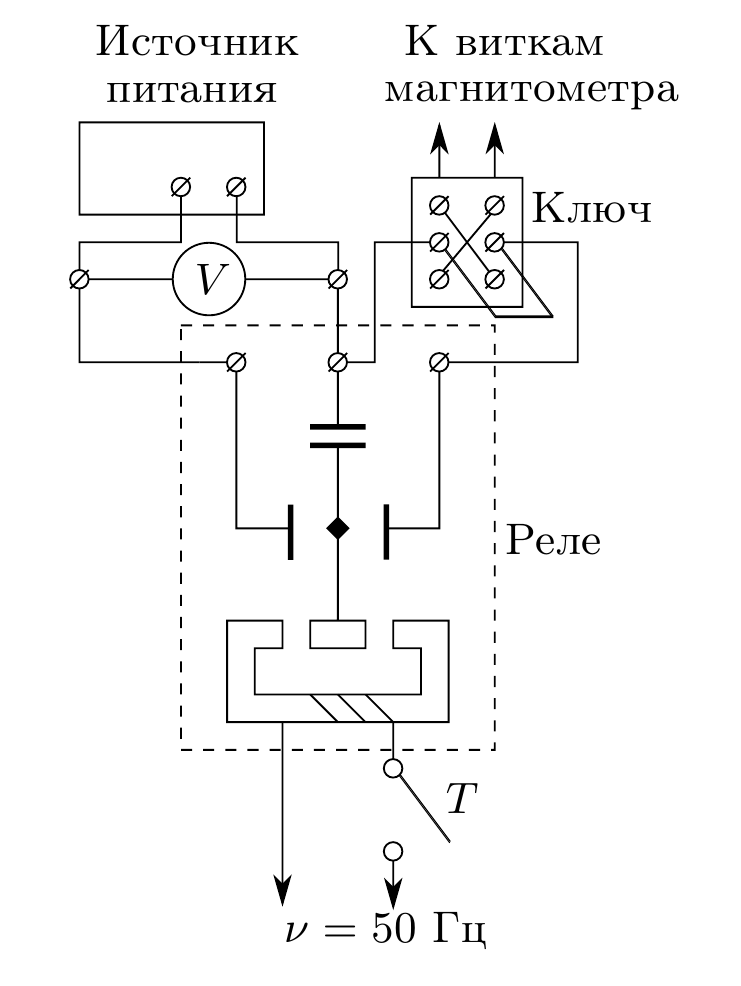
\includegraphics[scale=2.8]{3.png}
\end{center}
\caption{Схема питания катушки магнитометра}
\label{ris3}
\end{figure}

Таким образом, абсолютное измерение тока сводится к нахождению величин $C$ и $U$, которые тоже могут быть определены абсолютным образом. Так, ёмкость плоского конденсатора можно вычислить из его размеров, то есть опираясь только на единицу длины. Разность потенциалов также может быть определена абсолютным образом, например, через силу, действующую на пластину заряженного конденсатора, как это делается в абсолютном вольтметре. Мы, однако, не будем полностью проводить эту программу, а ограничимся только указанием на возможность её выполнения.

Итак, для вычисления абсолютного значения тока по \eqref{averamper} необходимо измерить напряжение $U$ на конденсаторе известной ёмкости $C$. Напряжение необходимо выразить в единицах СГС (измерительные приборы, как правило, проградуированы в единицах СИ: $1~B \approx \frac{1}{300}~ед.~СГС$). Ёмкость конденсатора $C$ [см] должна быть выражена в сантиметрах ($1~Ф \approx 9 \cdot 10^{11}~см$).

По отношению численных значений одного и того же тока, выраженных в единицах СИ и СГС (гауссовой) по формулам \eqref{amperage} и \eqref{averamper} соответственно, можно определить значение электродинамической постоянной:
\begin{equation}\label{electroconst}
c~\left[\frac{м}{c}\right] = \frac{1}{10}\frac{I_{[СГС]}}{I_{[СИ]}}.
\end{equation}

\section{Используемое оборудование}

\begin{enumerate}
    \item магнитометр;
    \item осветитель со шкалой;
    \item источник питания;
    \item вольтметр;
    \item электромагнитный переключатель;
    \item конденсатор;
    \item намагниченный стержень;
    \item прибор для определения периода крутильных колебаний;
    \item секундомер;
    \item рулетка;
    \item штангенциркуль.
\end{enumerate}

\section{Результаты измерений и обработка данных}

\begin{table}[h!]
\begin{center}
\begin{tabular}{|c|c|c|c|c|c|c|c|c|}
\hline
$n$ & $\nu_{т}, кГц$ & $a_{т}$ & $норм(a_{т})$ & $\nu_{изм}, кГц$ & $\delta_{\nu_{изм}}, кГц$ & $a_{изм}, мВ$ & $\delta_{a_{изм}}, мВ$ & $норм(a_{изм})$ \\ \hline
1 & 1 & 144,51 & 8,81 & 1,00 & 0,02 & 820 & 2 & 8,54 \\ \hline
2 & 2 & 128,76 & 7,85 & 2,00 & 0,02 & 736 & 2 & 7,67 \\ \hline
3 & 3 & 104,80 & 6,39 & 3,00 & 0,02 & 600 & 2 & 6,25 \\ \hline
4 & 4 & 75,68 & 4,62 & 4,00 & 0,02 & 432 & 2 & 4,50 \\ \hline
5 & 5 & 45,02 & 2,75 & 5,00 & 0,02 & 264 & 2 & 2,75 \\ \hline
6 & 6 & 16,39 & 1 & 6,00 & 0,02 & 96 & 2 & 1 \\ \hline
\end{tabular}
\end{center}
\caption{Результаты теоретического расчёта и измерений амплитуд и частот первых 6 гармоник спектра}
\label{tab1}
\end{table}

\section{Обсуждение результатов и выводы}

В данной работе был исследован спектральный состав периодических электрических сигналов.

При исследовании спектра периодической последовательности прямоугольных импульсов при фиксированных параметрах $\nu_{повт}$ и $\tau$ были измерены амплитуды и частоты первых 6 гармоник (таб.~\ref{tab1}). Измеренные значения соответствуют рассчитанным теоретически. Также была измерена зависимость ширины спектра $\Delta{\nu}$ от времени импульса $\tau$. Из полученной зависимости (рис.~\ref{plot1}) следует: $$\Delta{\nu} \cdot \tau \backsimeq 1,01\pm0,01,$$ что соответствует соотношению неопределённостей в рамках погрешности. Основной вклад в погрешность вносит определение коэффициента зависимости, так как благодаря использованию цифровых приборов другие источники погрешности отсутствуют или их влияние несущественно.

При исследовании спектра периодической последовательности цугов была измерена зависимость расстояния $\delta{\nu}$ между соседними спектральными компонентами сигнала от периода $T$ повторения импульсов. Из полученной зависимости (рис.~\ref{plot2}) следует: $$\delta{\nu} \cdot \tau \backsimeq 0,95\pm0,01,$$ что близко к соотношению неопределённостей. Здесь основной вклад в погрешность также вносит определение коэффициента зависимости.

При исследовании спектра амплитудно-модулированного сигнала была измерена зависимость отношения $a_{бок}/a_{осн}$ амплитуд боковой и основной спектральных линий от глубины модуляции $m$. Из полученной зависимости (рис.~\ref{plot3}) следует: $$\frac{a_{бок}}{a_{осн}} = 0,510\pm0,004 \cdot m,$$ что соответствует теоретической зависимости $\frac{a_{бок}}{a_{осн}} = \frac{m}{2}$. Аналогично здесь основной вклад в погрешность вносит определение коэффициента зависимости.

Также в данной работе был изучен спектр сигнала, модулированного по фазе. Спектры сигналов при различном максимальном отклонении $\varphi_m$ приведены на рис.~\ref{ris24}-\ref{ris25}.

\end{document}
